\section{Microservices}

Microservice is a specialized implementation of Service Oriented Architecture(SOA) \cite[chapter ~3]{SOA}. A service in a SOA
is a functional unit that performs a specific business action (e.g. user authentication) accessed typically via a network that 
encapsulates its state and the operations performed on the data.  
Figure \ref{fig:objectBasedDS} illustrates an example of Service Oriented Architecture (SOA) in a distributed system where different services call each others interface
to perform a certain action. Although microservices are built using the SOA paradigm, they have their differences. In a microservice, a service can be deployed and 
operated independently because the services are designed to be more fine grained with a single purpose, unlike SOA. 
Also they are lightweight and Domain Driven \cite{DDD} that makes the application simple to understand, develop, and test. The smaller set of services
can be developed autonomously by different teams and be deployed quickly as they usually are lightweight in nature. This architecture promises to bring loose coupling 
by separating a big application into smaller logical units. 


\begin{figure}[H]
    \centering 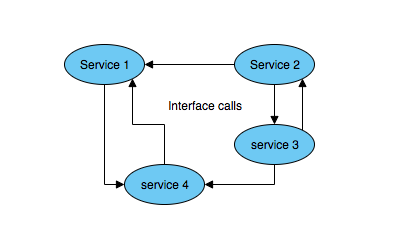
\includegraphics[scale=0.7]{grafiken/objectBasedDS.png}
    \caption{An service oriented architecture in a distributed system 
        \cite[p.~62]{DistributedSystems}}
    \label{fig:objectBasedDS}
\end{figure}


Figure \ref{fig:serviceExample} shows an example of how 
a service is domain bounded and there is a flexibility of choosing different
technologies for the isolated services \cite{MicroserviceNewMan}. 
Each service is encapsulated with their own life cycles, which communicates with each other using protocols 
(e.g. HTTP \cite{HTTP}, websockets \cite{WebSockets}, GRPC \cite{grpc}). 

\begin{figure}[H]
    \centering 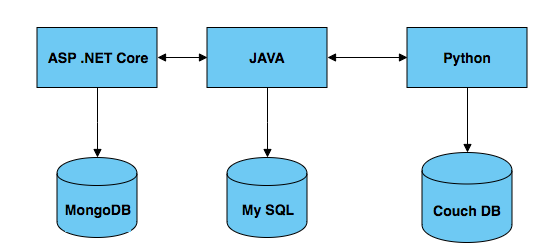
\includegraphics[scale=0.6]{grafiken/microservices.png}
    \caption{ Illustration of services as fine grained independent entities}
    \label{fig:serviceExample}
\end{figure}

    

\par
    A single monolithic application \cite[p.~94]{{softwareDesign}} is
    built as a large unit where all the logic lies within a single system. 
    This is considered the most natural way to develop a server-side 
    application. It is seen that as the application scales in size, it 
    gets harder to keep up with the changes as scaling requires an entire
    system to be scaled. This is where microservices can be beneficial,
    as only the required bounded module can be scaled up as needed. 
    There are different factors to be considered before going for a microservice
    architecture as improper planning could lead to an unstable system.

    \begin{table}[h!]
        \centering
        \begin{tabular}{|p{7.3cm}|p{7.3cm}|}
            \hline
                \textbf{Advantages}  & \textbf{Disadvantages}\\
            \hline
                The services can be developed with different languages & 
                A mature team must be present to maintain large number of services \\
            \hline
                A strong modular boundaries is present which reinforces a modular
                structure.
                & All the services must manage data consistency amongst the services which is
                harder to manage in a large distributed system.\\
            \hline
                 Independent deployment is easier since the services are
                 autonomous. & Harder to program since remote calls must be made.\\
            \hline
        \end{tabular}
        \caption{Advantages and disadvantages of microservices \cite{FowlerMartin}}
        \label{table:Advantages and disadvantages of microservices}     
    \end{table}    

    \newpage
    \subsection{Data Sovereignty in Microservice}
    \label{subsection:dataSovereignty}
    It is an important guideline for a microservice architecture to own its domain data and 
    logic \cite[p.~29]{Torre2017}. Decentralized data would assist a individual microservice
    to become solely independent and help them evolve separately. The approach of each microservice owning its own database is also
    know as \textbf{Polyglot Persistence} \cite{Polyglot}. Applying this pattern would imply that the
    data belonging to one service is available to the others only via the API of the microservice.

    \begin{figure}[H]
        \centering 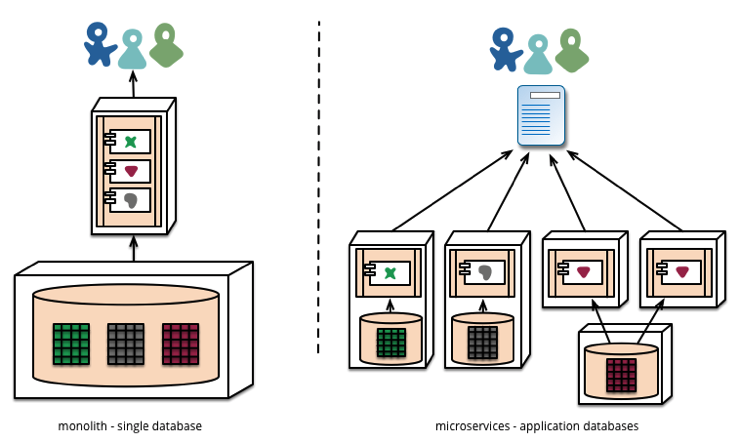
\includegraphics[scale=0.4]{grafiken/polyglot.png}
        \caption{Data management approach in a Monolithic application vs microservice \cite{FowlerMartin}}
        \label{fig:polyglot}
    \end{figure}
    
   In Figure \ref{fig:polyglot}, it can be observed how a Monolithic application owns only a single database for the whole application. Meaning,
   the application has a centralized database which are shared amongst the services. Whereas, in microservices each service owns
   a single database or few services share databases which is easier to manage. Having said that data sovereignty is very beneficial, it also brings various difficulties
   i.e. coordinations between services, which is very challenging to tackle and creates data coherency issues in the system. 




